\chapter{Desenvolvimento} \label{cap:desenvolvimento}


\section{Software}
Nesta seção serão discutidas as implementações realizadas na parte dos serviços executados em nuvem, como servidor em Python, Banco de dados e Página Web e o aplicativo local em Android passando por uma visão geral do funcionamento de cada parte além da comunicação entre os três softwares envolvidos e a comunicação embarcada.


\subsection{\textbf{Sistema Web}}

A interface \textit{Web} foi desenvolvida utilizando linguagem de marcação HTML com o auxilio das bibliotecas \textit{Bootstrap} para auxilio na construção da interface e \textit{JQuery} para manipulação de \textit{DOM}. O \textit{JQuery} é responsável por fazer as requisições HTTP ao servidor para a aquisição dos dados de população dos gráficos.

\subsubsection{Protocolo de comunicação}

Toda a comunicação é feita utilizando o protocolo HTTP. A página web executa uma requisição para um endpoint do servidor.

 Um endpoint é o final de um canal de comunicação, quando nossa aplicação se comunica com outro sistema como o aplicativo Android ou o sistema Web, os pontos onde se realiza o contato dessa comunicação são chamados de endpoints, para nossa aplicação o endpoint seria a URL de contato entre o servidor e o agente de contato trabalhando em formato de requisição e resposta, ou seja, nossa aplicação se comunica com o servidor e espera sua resposta para dar continuidade à sua execução. As requisições feitas na interface são de forma assíncrona e após o retorno são chamados os métodos que populam as informações para o gráfico. A Figura 26 demonstra como é feita a população das informações.


 \begin{figure}[H]

\begin{center}
     \caption{Fluxo de população de informação }
  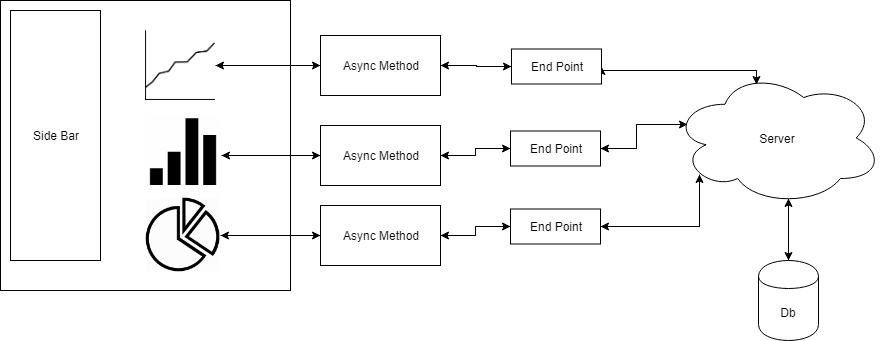
\includegraphics[width=150mm]{images/Cap4/cap_4_servidor.png}
\end{center}
 \scriptsize Fonte: Os autores
  
\end{figure}

Com a Figura 26 é possível notar que cada gráfico ou tabela presente na página \textit{web} possui seus métodos próprios de comunicação sendo chamados os \textit{endpoints} do servidor de forma assíncrona e com isto cada gráfico recebe seu tipo de dado tratado e formatado para o rápido carregamento das informações.

\subsection{\textbf{Aplicação}}

O aplicativo foi desenvolvido utilizando Java como linguagem base, voltado ao Android 4.3 ou superior, de forma a comportar o máximo de usuários possíveis. O aplicativo possui um banco de dados em \textit{SQlite} para guardar informações essenciais do usuário, como o login de cadastro no celular e \textit{token} do \textit{Firebase}.

No projeto foi utilizado o serviço \textit{Firebase Cloud Messaging} ou FCM disponibilizado pela \textit{Google} sendo  responsável pelo sistema de aviso dos usuários para poder utilizar o serviço é necessário armazenar o \textit{token} fornecido pela FCM para a identificação do usuário pois este \textit{token} é a chave única do usuário, com isto é possível monitorar e alertar usuários específicos do sistema.


Para poder manter o serviço de monitoramento funcionando, mesmo que o aplicativo seja fechado, foi criado um canal de notificação que é responsável por definir o comportamento do aplicativo tanto visual como auditivo sendo responsável por criar os \textit{pop-ups} de notificações no aparelho.

 Dentro deste canal de notificação são gerados serviços pela aplicação em primeiro plano que é executada após se logar e conectar pela primeira vez no \textit{Bluetooth}.
 Estes serviços são responsáveis por executar métodos recursivos para o monitoramento do canal de comunicação \textit{Bluetooth} e os sensores presentes no \textit{Android}.



\subsubsection{Serviços da aplicação}

O principal objetivo do aplicativo é manter todos os serviços necessários em execução mesmo que o usuário o finalize, para manter a aplicação sendo executada foi  utilizado um serviço em primeiro plano.

Quando o usuário se conecta  pela primeira vez o serviço é instanciado e executado,e  quando o usuário finaliza a aplicação o serviço que foi criado não é finalizado, quando o usuário instância uma nova aplicação  o serviço que foi executado por uma instância anterior do aplicativo é vinculado a uma nova instância do aplicativo.Isso faz com que o Android reaproveite sua antiga instância na nova. A Figura 27 demonstra um ciclo de vida de um serviço. 

De forma geral o serviço é um componente da aplicação que realiza execuções sem a necessidade da interface do usuário. Mesmo que seja instanciado uma nova aplicação  o serviço criado continuará em execução em segundo plano.


Por fim, quando um serviço é vinculado a um aplicativo  é gerada uma interface cliente-servidor para que os métodos se comuniquem com a aplicação.  O serviço vinculado permanece em execução enquanto uma aplicação estiver vinculada a ele, mesmo finalizando a instância da aplicação o serviço continuará vinculado. Após a criação de uma nova instância da aplicação, o serviço vinculado à instância anterior é reaproveitado pelo sistema, o serviço será eliminado caso todos suas instâncias sejam desvinculadas pelo aplicativo.

 \begin{figure}[H]

\begin{center}
     \caption{Ciclo de vida de um serviço }
  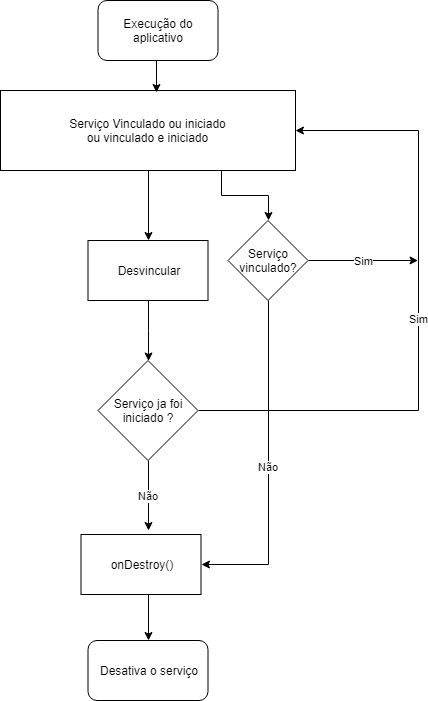
\includegraphics[width=80mm]{images/Cap4/Servicos_android.png}
\end{center}
 \scriptsize Fonte Os autores
  
\end{figure}



Dentro dos serviço gerados  são iniciados os \textit{listeners} dos sensores e o canal de comunicação.
O \textit{listener}  é definido como uma interface  que  "escuta"  o evento definido no \textit{script} e dependendo do que é recebido, é executada uma ação. Este evento pode ser considerado uma interrupção do sistema, pois fica escutando paralelamente e, quando recebe a informação, gera uma interrupção no aplicativo para executar seus métodos.

A partir deste momento todos os módulos atuam de forma individual dentro do aplicativo com seus respectivos \textit{listeners} . A Figura 28 demonstra os métodos utilizados

 \begin{figure}[H]

\begin{center}
     \caption{\textit{Listeners}}
  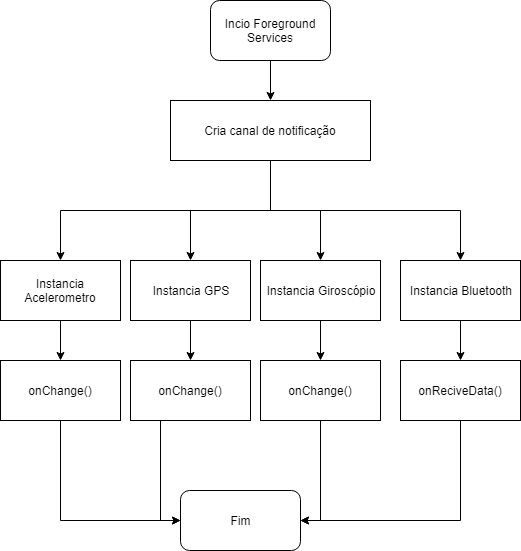
\includegraphics[width=100mm]{images/Cap4/notificao_android.png}
\end{center}
 \scriptsize Fonte: Os autores   
  
\end{figure}



\subsubsection{Protocolo de comunicação com o Servidor}

Para realizar a comunicação entre o aplicativo e o Servidor será enviado um pacote de dados em formato \textit{JSON} com codificação UTF-8  contendo as informações necessárias de identificação do usuário. Quando este pacote chega ao Servidor ele irá validar se o  usuario existe na base com as informações recebidas no pacote de informação, caso o registro do usuário não exista no banco de dados o Servidor irá retornar uma mensagem de que o usuário não foi encontrado para o aplicativo, quando o registro é encontrado  o Servidor irá executar o método requisitado pelo aplicativo definido pela URL de requisição retornando status 200 e com um pacote de dados em formato \textit{JSON} com codificação UTF-8 para o aplicativo.


\subsubsection{Protocolo de comunicação com o Embarcado}

Para o Android foi utilizado o \textit{Bluetooth} Standard como meio de comunicação do embarcado dentro de um serviço em primeiro plano. Dentro deste serviço foi criado uma classe responsável por gerenciar toda a comunicação com o embarcado. Esta classe possui atributos de conexão do \textit{Android}, o contexto da aplicação, sendo que o contexto é definido por quem está chamando a execução da classe e os métodos de \textit{listeners } do \textit{Bluetooth} como \textit{onDataReciver()} responsável por receber a informação do embarcado e enviar as informações para o Servidor utilizando Protocolo HTTP com o método POST. E, por fim,  os \textit{listeners } de conexão sendo responsáveis por monitorar se conectou corretamente, se desconectou, ou se a conexão falhou forçando uma nova  reconexão com 5 tentativa. Após isso o aplicativo desabilita o módulo \textit{Bluetooth} e continua operando somente com os sensores do celular.


\subsection{\textbf{Servidor}}

O servidor foi construído utilizando \textit{Python} 3.6.8 com o banco relacional   \textit{PostgreSQL},com as  especificações técnicas sistema operacional \textit{Ubuntu}  18.04, processador \textit{Intel Xeon} 2.2GHz, 1 \textit{Gigabyte}  de memória RAM e 40 \textit{Gigabyte} de espaço de armazenamento.

Com estas especificações técnicas foi desenvolvida uma aplicação em \textit{Python} utilizando a biblioteca \textit{HTTPserver}, responsável por criar um servidor socket TCP para escutar e gerenciar as requisições recebidas. Também utiliza bibliotecas como \textit{pandas}, responsável pela manipulação de estrutura dos dados recebidos pelo banco; \textit{psycopg2}, responsável pela conexão e comunicação entre o servidor \textit{Python}; e o banco relacional \textit{PostgreSQL}, \textit{FirebaseAdmin} sendo a classe de comunicação do serviço da \textit{Google}; e, por fim, a biblioteca \textit{pyowm}, responsável por adquirir as informações climaticas.

Além disto o Servidor possui um \textit{Apache} sendo executado na porta 80 como  um serviço do Ubuntu sendo responsável pela pagina \textit{Web}.


\subsubsection{Firebase}

Quando uma requisição de acidente chega ao  servidor, será executada uma consulta no banco procurando todos os usuários ativos a partir da última hora. Com esta listagem de usuários será feito um cálculo individual de distância de cada usuário ativo em relação à vítima. Caso algum usuário ativo esteja dentro do \textit{threshold} estabelecido ele será adicionado em uma nova listagem de usuários que serão notificados. A partir disto é executada a classe do \textit{Firebase} assinando todos estes usuários em um tópico único e logo em seguida é enviado um pacote de informação em formato \textit{JSON} para o \textit{Firebase} com o tópico registrado e a respectiva mensagem que o usuário vai receber. Logo após o envio do \textit{Firebase} é executado uma inserção no banco para registrar o ocorrido passando as informações de localização, horário, vítima, e clima para o banco de dados.

Foi necessário fazer este cálculo de proximidade pois o limite de membros que podem estar no mesmo tópico é de mil  usuários. A Figura 29 demonstra o funcionamento do \textit{Firebase}.

 \begin{figure}[H]

\begin{center}
     \caption{Fluxo de envio do Firebase }
  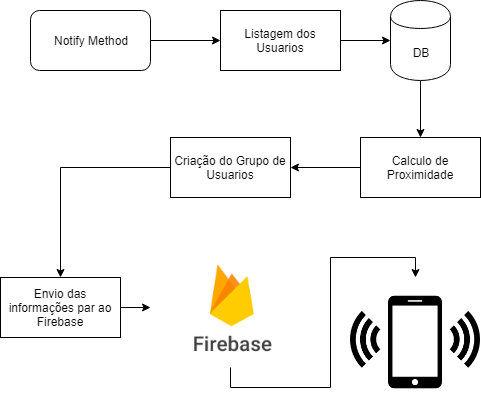
\includegraphics[width=120mm]{images/Cap4/cap_4_firebase_fluxo.png}
\end{center}
 \scriptsize Fonte: Os autores
  
\end{figure}


\subsubsection{Banco de dados}

Durante o desenvolvimento do projeto foi modificada a estrutura do banco para atender à aplicação. Com isto foi desenvolvido um novo esquema do banco, reduzindo a quantidade de relacionamento entre tabelas, aumentando a performance do sistema. A Figura 30 representa o novo diagrama do banco de dados.

 \begin{figure}[H]

\begin{center}
     \caption{Diagrama do Banco de dados}
  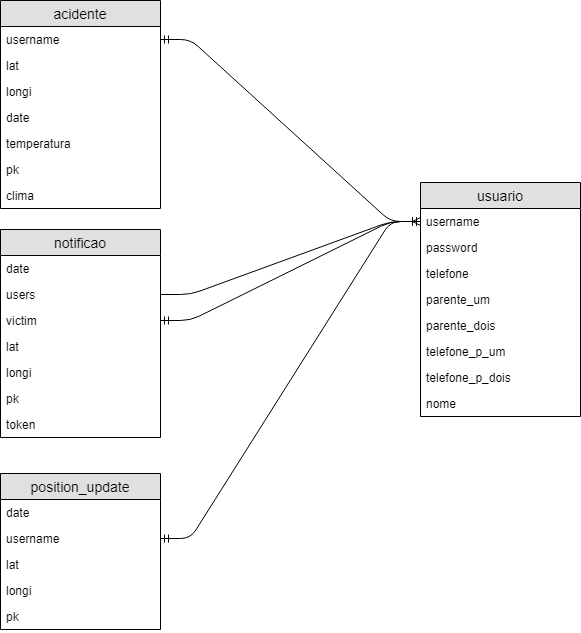
\includegraphics[width=100mm]{images/Cap4/diagrama_banco.png}
\end{center}
 \scriptsize Fonte: Os autores
  
\end{figure}


\section{Sistema Embarcado}
 O desenvolvimento do sistema embarcado utilizou o ambiente do Arduino IDE, auxiliado de bibliotecas C/C++, responsáveis por implementar as comunicações do protocolo I2C, e \textit{Bluetooth Classic}, além de permitirem um acesso mais direto às informações do módulo MPU.
 
Com o desenvolvimento foi identificado que o \textit{Bluetooth Low-Energy} não se comportou da forma idealizada, causando algumas incompatibilidades com o aplicativo \textit{Android}. A utilização do BLE também se monstrou restritiva quanto aos \textit{Smartphones} utilizados, pois se faz necessária uma versão mais elevada e recente da tecnologia, o que pode ser um impeditivo quanto ao público alvo. Tendo em vista esses pontos foi optado pela utilização do \textit{Bluetooth Standard} . 

\subsection{\textbf{Hardware}}

O \textit{hardware} foi desenvolvido de forma que a ESP-32 (microcontrolador) troque informações com o MPU-6050 (circuito integrado com os sensores) utilizando  comunicação digital. Como ambas utilizam o protocolo I2C, o mesmo foi utilizado.
Além das conexões SCL e SDA necessárias para o protocolo, também foi utilizada uma conexão extra para interrupção. Essa interrupção é gerada pelo DMP presente no MPU e sinaliza toda vez que um bloco de informações foi processado e está disponível para leitura.

As \textit{GPIOs} utilizadas foram selecionadas conforme a capacidade da ESP-32, mais especificamente o modelo NODE MCU 32-S, e o posicionamento mais adequado para o circuito.

O conversor DC-DC \textit{buck} utilizado alimenta o circuito com 5V e apresenta  boa eficiência. Essa eficiência faz com que uma pequena parte da tensão rebaixada seja convertida em calor, o que reduz a temperatura do sistema embarcado.
O circuito apresenta-se na figura 31.

 \begin{figure}[H]

\begin{center}
     \caption{Circuito do sistema embarcado }
  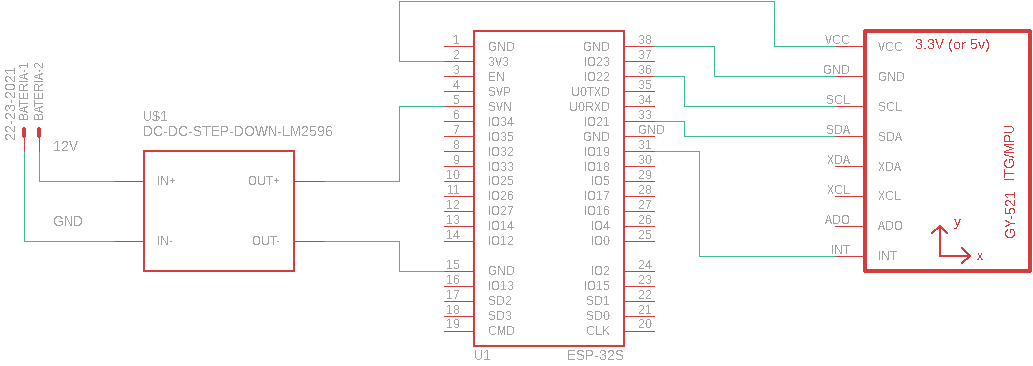
\includegraphics[width=150mm]{images/Cap4/Esquema_esp.png}
\end{center}
 \scriptsize Fonte: Os autores
  
\end{figure}




Para a construção da caixa de armazenamento do circuito no veículo foi utilizada uma impressora 3D. Com o modelo base  encontrado no \textit{thingiverse}, um site que contém modelos e criações para impressão 3D, houve a necessidade de modificação e escala do objeto para comportar o circuito e o material escolhido para absorção de impacto. A modificação da caixa foi realizada utilizando o \textit{software} 3DBuilder e consistiu no redimensionamento dos eixos X, Y e Z. Como o redimensionamento direto afeta todo o modelo, foi necessário refazer a furação dos parafusos utilizando os cilindros disponíveis no programa.

A caixa final possui as dimensões de 14x8x3.5cm, o que comporta todo o circuito e contém espaço para o material anti-impacto. Para testes o material anti-impacto escolhido foi espuma por ser de fácil acesso, além do envolvimento da placa de circuito em plástico bolha. A caixa foi fechada e vedada com cola, possuindo ao fim proteção contra respingos e chuva, porém devido a forma de impressão da caixa a mesma não é prevista que fique submersa. A caixa em questão é demonstrada na figura 32.

 \begin{figure}[H]

\begin{center}
     \caption{Caixa impressa}
  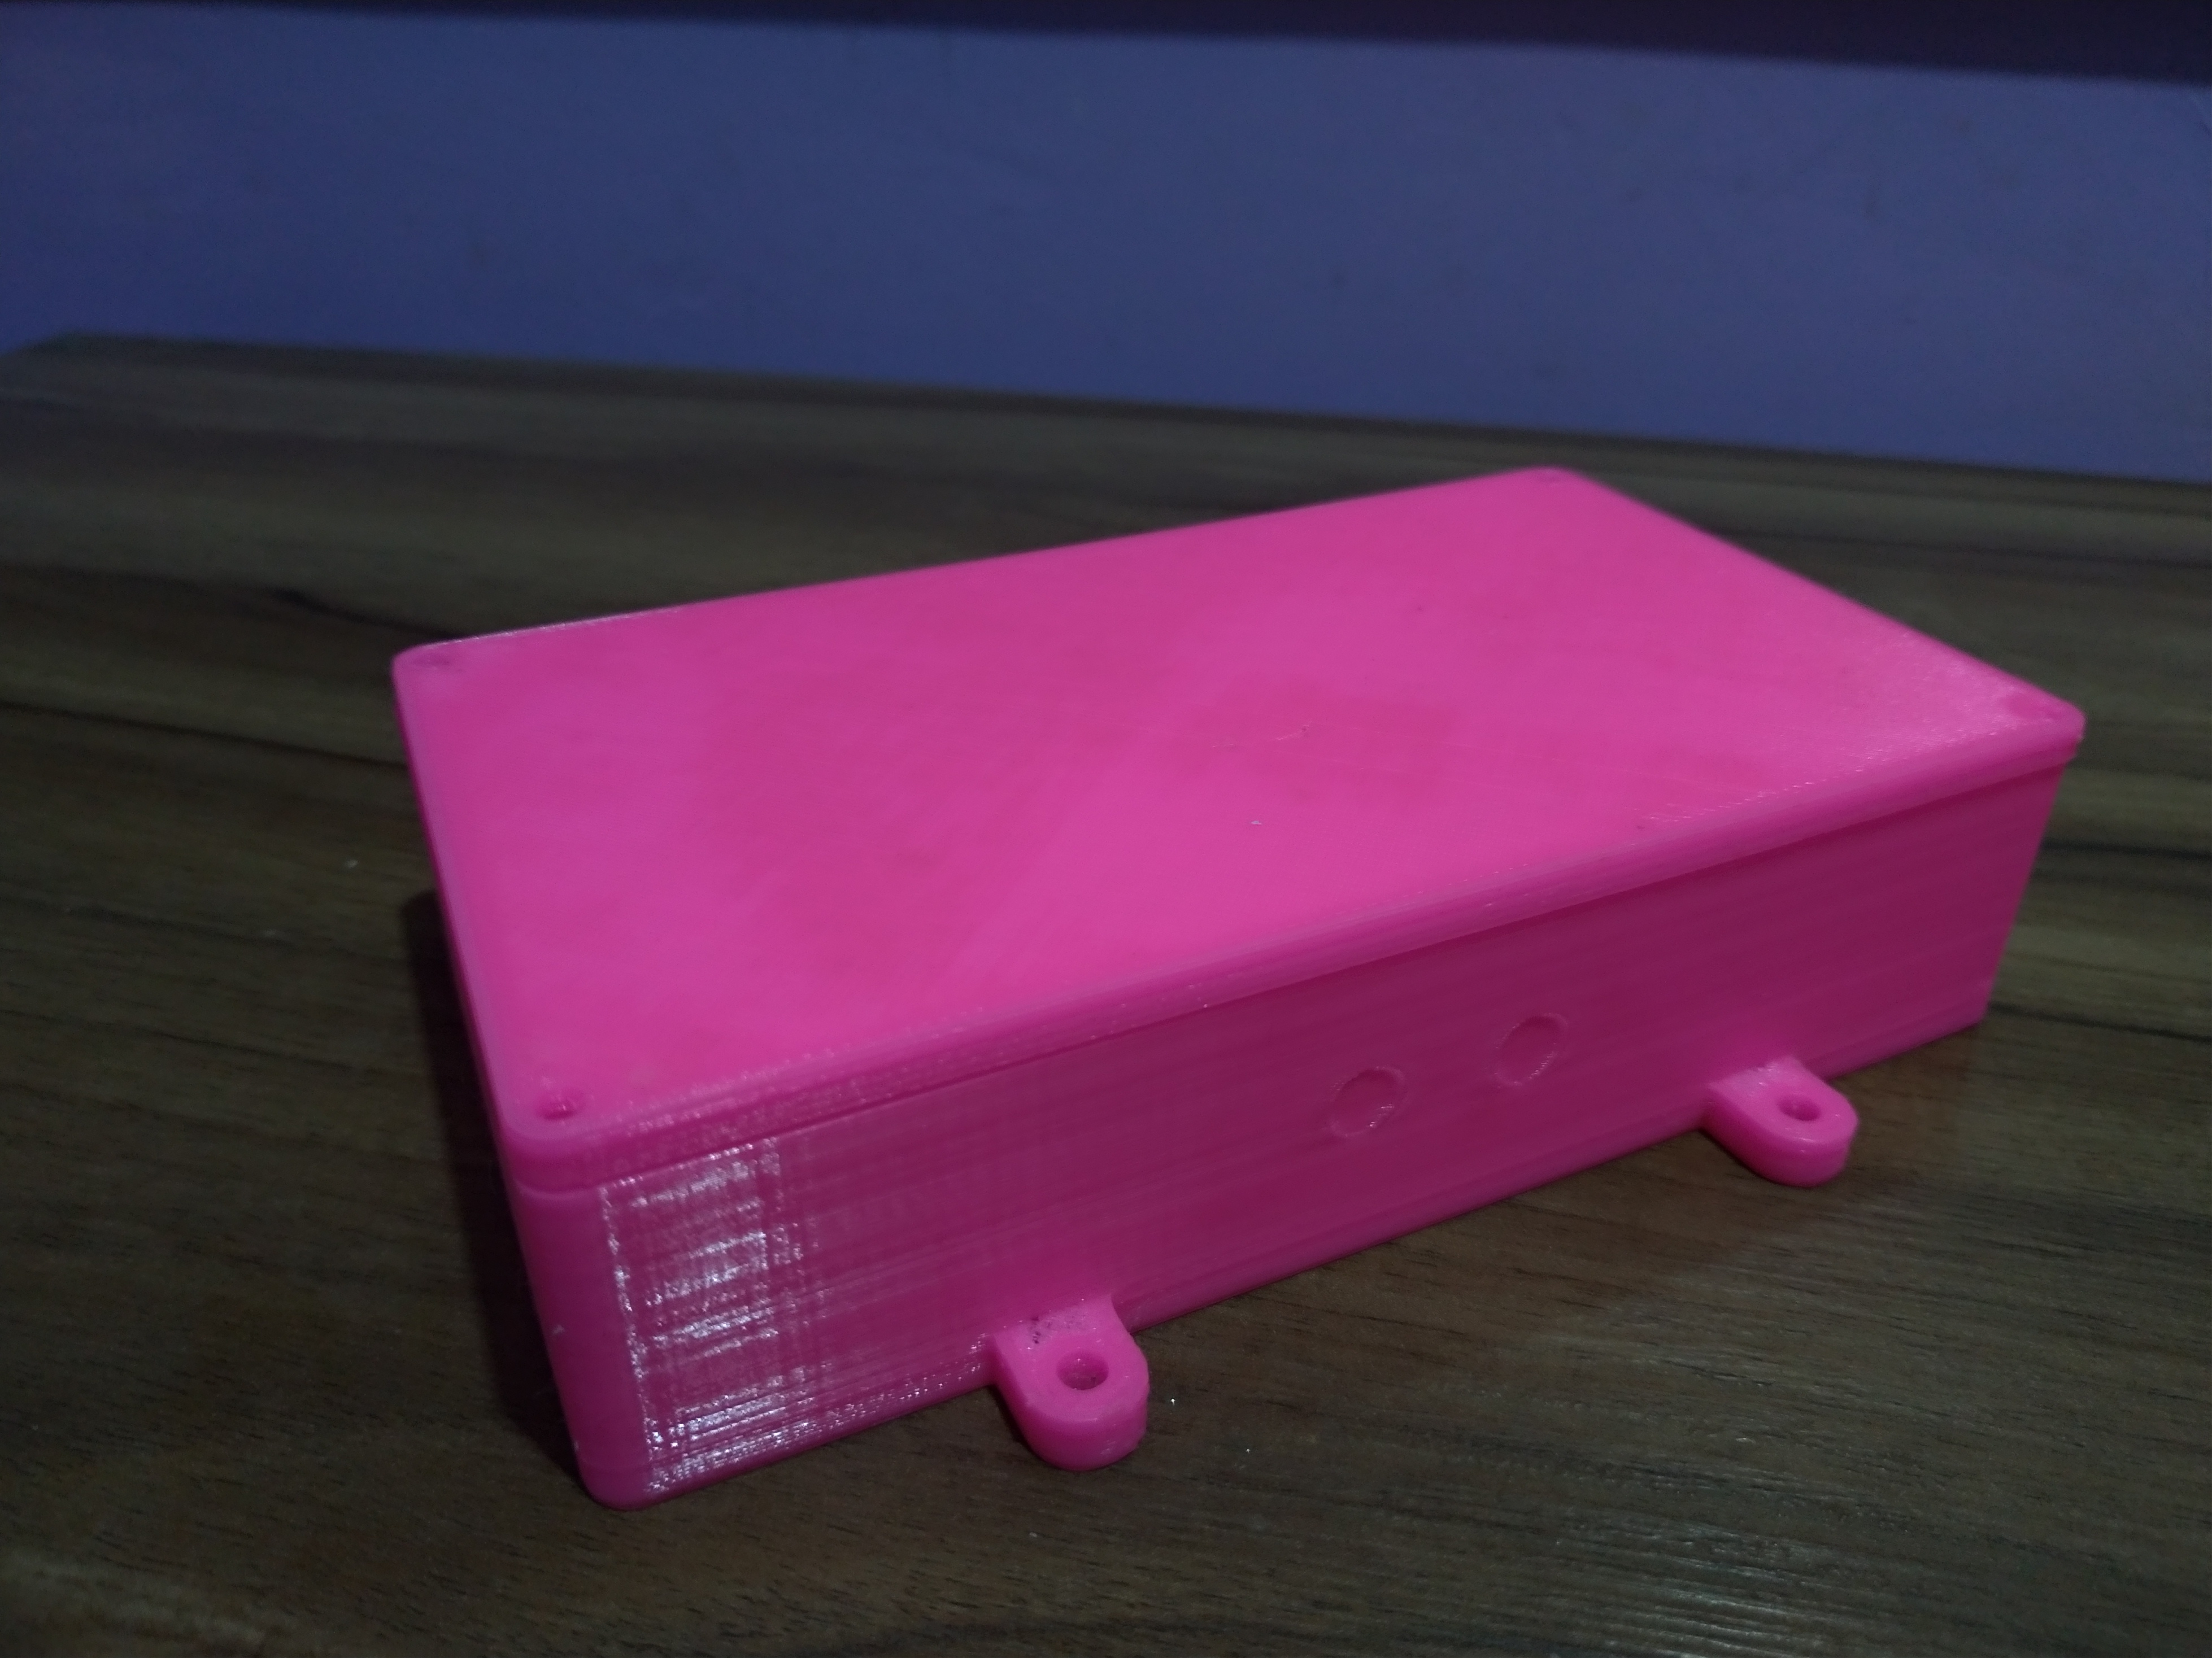
\includegraphics[width=150mm,height=100mm]{images/Cap4/caixa_tampa.jpg}
\end{center}
 \scriptsize Fonte: Os autores
  
\end{figure}

\subsection{\textbf{Firmware}}

O \textit{firmware} foi desenvolvido com o auxilio de bibliotecas para comunicação I2C e \textit{Bluetooth} e tem como função notificar o aplicativo \textit{Android} da detecção de acidentes.

O desenvolvimento do \textit{firmware} é comentado abaixo.


\subsubsection{Posicionamento e aceleração}
Os eixos X, Y e Z do acelerômetro e giroscópio presentes no MPU-6050 são fixos e relativos ao módulo de forma similar ao apresentado no \textit{smartphone}. Por exemplo o eixo vertical Z do módulo é equivalente ao eixo Z do \textit{smarphone}, este o qual é perpendicular a tela do aparelho.

Como o sistema embarcado deve ser fixado sempre na vertical com a mesma orientação, faz-se desnecessária a obtenção do ângulo referente ao eixo Y, uma vez que este varia confome a movimentação do motociclista. Dessa forma, os eixos X (\textit{pitch}) e Z (\textit{roll}) são os eixos utilizados para analisar o comportamento do motociclista .

A força de impacto é obtida a partir do cálculo da resultante entre os três eixos (X, Y e Z) do acelerômetro. Essa abordagem possibilita colocar pesos para cada eixo, sendo o eixo Y menos significativo (é presente a força de aceleração da gravidade) e o eixo Z o mais significativo (registro de acidentes com colisão frontal). Os pesos para os eixos foram obtidos de forma empirica, obtendo-se então 1, 0.7 e 1.2 para X, Y e Z respectivamente.


\subsubsection{Configuração e parametrizações}

Inicialmente é configurada a utilização da comunicação I2C segundo os parâmetros de funcionamento da ESP32, o que permite a posterior utilização do módulo MPU. Com a correta parametrização da comunicação é, então, instanciado o objeto responsável por gerir o MPU, chamando sua função de inicialização.

Com a instanciação do objeto MPU, faz-se, inicialmente, uma verificação de comunicação para garantir a correta inicialização do I2C. Em seguida é também inicializada a utilização do DMP e a configuração de \textit{offset} dos eixos do acelerômetro e giroscópio. Estes offsets foram obtidos a partir dos exemplos de utilização da biblioteca do MPU e são únicos para o módulo. Para finalizar a configuração do MPU é, então. realizada a calibração dos eixos do acelerômetro e giroscópio e configuração da interrupção para cada obtenção de valores. Com esses procedimentos realizados é possível, então, chamar a função que habilita o DMP (permite o cálculo de movimentos complexos pelos eixos).

A ultima etapa de configuração corresponde a inicialização do \textit{Bluetooth}, sendo necessário instanciar e inicializar o objeto com o nome de identificação desejado.



\subsubsection{Funções e lógica de funcionamento}

A função de interrupção conta apenas com um contador, que tem seu valor somado a cada finalização de leitura do módulo MPU e subtraído a cada processamento desses valores pelo \textit{firmware}.

O processamento das interrupções ocorre em na função \textit{main} e se dá pela chamada de uma função responsável pela obtenção dos valores do módulo MPU. Utilizando a biblioteca, é requisitada a leitura dos valores de acelerômetro e giroscópio. Normalmente as funções da biblioteca necessitam de parâmetros adicionais, como a aceleração da gravidade que é obtida a cada nova leitura do módulo.

Uma vez que esses valores sejam lidos e armazenados em variáveis globais é, então, obtido o valor absoluto máximo entre os eixos X e Z. Em seguida, é calculada a resultante entre os eixos do aceletrômetro com seus devidos pesos.

Na função \textit{main} são verificados os valores resultantes obtidos da função de leitura. Se estes valores ultrapassarem limites pré-determinados é então determinada a ocorrência de um acidente.  Com esta ocorrência determinada, é verificada a conexão do dispositivo \textit{Bluetooth} buscando pelo pareamento. Se o aplicativo \textit{Android} estiver pareado um sinal de alerta é enviado, finalizando a operação do \textit{firmware}.

Os valores utilizados para a classificação de acidentes (aceleração e ângulo máximos) são discutidos no capítulo de testes e resultados.


